\documentclass[10pt]{article}

% Minimal packages for fast compile
\usepackage{times}
\usepackage[utf8]{inputenc}
\usepackage[T1]{fontenc}
\usepackage[a4paper,margin=2cm]{geometry}
\usepackage{titlesec}
\usepackage{graphicx}
\usepackage{booktabs}
\usepackage{float}
\usepackage[section]{placeins}
\usepackage{setspace}

% Section title styles
\titleformat{\section}{\bfseries\fontsize{12}{14}\selectfont}{\thesection.}{0.5em}{}
\titleformat{\subsection}{\bfseries\fontsize{11}{13}\selectfont}{\thesubsection.}{0.5em}{}

% Custom title page
\begin{document}

\begin{titlepage}
\centering
\vspace*{2cm}

\includegraphics[width=0.3\textwidth]{image.png}
\vspace{1cm}

{\Huge\bfseries Project Plan\par}
\vspace{2cm}

\begin{flushleft}
\textbf{Name of submission:} Project Plan\\[0.5em]
\textbf{Group name:} Testbench for Bit-Serial RISC-V processor in SoI for Venus\\[0.5em]
\textbf{Date:} 2025/10/13\\[0.5em]
\textbf{Organization:} KTH\\[1.5em]
\textbf{Authors:}\\[0.5em]
\begin{center}
\begin{tabular}{p{5cm}p{6cm}}
\toprule
\textbf{Name} & \textbf{Email} \\
\midrule
Chinmay Purandare & \texttt{chinmayp@kth.se} \\
Lorenzo Parata & \texttt{parata@ug.kth.se} \\
Chongnan Wang & \texttt{chongnan@kth.se} \\
Xiaotian Jiang & \texttt{xjia@kth.se} \\
Xinxin Qin & \texttt{xinxinq@kth.se} \\
Paul Martin & \texttt{paulmart@kth.se} \\
\bottomrule
\end{tabular}
\end{center}
\vspace{1em}
\end{flushleft}

\vfill
\begin{flushright}
\textbf{Department of Electronics}\\
KTH Royal Institute of Technology\\
Stockholm, Sweden
\end{flushright}
\end{titlepage}

% Table of Contents on separate page
\clearpage
\tableofcontents
\thispagestyle{plain}
\clearpage

% Start main content
\section{Background}
This project continues previous work at KTH developing digital electronics for extreme high-temperature environments, specifically targeting Venus surface conditions. Last year's students successfully designed and synthesized two RISC-V processor variants—a parallel model in VHDL and a bit-serial CISC-V model in ProGram—both optimized for the 12-pad constraint of KTH's high-temperature test station. However, they did not complete FPGA implementation and testing.\\
The current project addresses this gap by implementing and testing both processor models on FPGAs, developing an advanced testbench on a separate FPGA, and integrating the multi-FPGA system to validate functionality. This work uses KTH's experimental Silicon-on-Insulator technology, which can operate at temperatures approaching Venus's 480°C requirement, and leverages the open-source RISC-V architecture to avoid licensing constraints.\\
The project requires expertise in hardware design, software development, FPGA implementation, and system integration, with support from supervisors Artur Podobas (RISC-V/compiler) and Johnny Öberg (ProGram/FPGA). Success will validate these designs for eventual ASIC fabrication and demonstrate processor viability for extreme-environment applications.

\section{Goal}

The main objective of this project is to design, implement, and validate an FPGA-based testbench system capable of verifying and comparing the functional correctness of two existing processor architectures—a standard RISC-V core and a novel Bit-Serial CISC-V core.  
While both processor architectures are already synthesized and available, their deployment serves primarily as a means to validate the testbench design and assess its verification capabilities rather than being the main focus of the project.  
The entire project will be completed within a 16-week timeframe using mature FPGA design environments and RISC-V toolchains to ensure measurable and demonstrable results.

\subsection{Project Goal}
The goal of the project is to develop a dual-FPGA prototyping and validation platform in which one FPGA hosts the processor-under-test (either RISC-V or CISC-V), while the other FPGA implements a general-purpose testbench.  
This testbench will include fundamental components such as a UART controller for communication with a host PC, a GPIO interface for interaction with the processor and peripheral emulation, and a memory unit for loading and executing test programs.  
The architecture of the testbench will be designed to be modular and general, allowing extensions or modifications in later development stages, but not necessarily representing the final verification infrastructure.

The verification process will follow multiple measurable phases:
\begin{itemize}
    \item Validation of both processor architectures using a suite of at least 10 assembly-level test programs to verify core ISA functionality.
    \item Execution and verification of a complex benchmark algorithm (e.g., CoreMark or matrix multiplication), with results transmitted to the host PC.
    \item Demonstration of stable data transfer exceeding 1,000 instructions without corruption between the two FPGAs.
    \item (Optional, non-priority) Collection of quantitative performance metrics such as maximum clock frequency (F\textsubscript{max}), benchmark cycle counts, and FPGA resource utilization (LUTs, FFs, BRAM) for comparative analysis.
\end{itemize}

\subsection{Business Goal}
The business goal of the project is to successfully complete all design, implementation, and validation phases within the planned 16-week schedule, strictly meeting all internal deadlines and course assignments.  
In addition to the technical objectives, the project aims to strengthen our teamwork, communication, and project management skills by maintaining an organized workflow, clear task distribution, and effective collaboration throughout all development phases.  
The final target is to deliver a high-quality, fully functional system and comprehensive documentation that meets all evaluation criteria and achieves a final project grade of \textbf{A}.

\section{Organization}

This section describes how our group is organized, including the members involved in the project, their responsibilities, and our internal work structure and communication methods.

\subsection{Project Members and Responsibilities}

The following table lists all project members together with their contact information and main responsibilities within the project.

\begin{table}[h!]
\centering
\begin{tabular}{|l|l|l|}
\hline
\textbf{Name} & \textbf{Email} & \textbf{Responsibility} \\ \hline
Chongnan Wang & chongnan@kth.se & Software development \\ \hline
Xinxin Qin & xinxinq@kth.se & ASIC design \\ \hline
Paul Martin & paulmart@kth.se & Hardware architecture \\ \hline
Xiaotian Jiang & xjia@kth.se & RISC-V verification \\ \hline
Chinmay Purandare & chinmayp@kth.se & Hardware architecture \\ \hline
Lorenzo Parata & parata@ug.kth.se & Software development \\ \hline
\end{tabular}
\caption{Project members and their responsibilities.}
\end{table}

Our group follows a consensus-based decision-making approach without a fixed project manager. Instead, responsibilities such as organizing meetings, keeping time, and moderating discussions rotate between members when necessary.  
In particular, Lorenzo Parata serves as process leader and moderator, ensuring smooth workflow and coordination among team members. Paul Martin acts as timekeeper, while Chongnan Wang, Xinxin Qin, and Xiaotian Jiang share the secretary role for documentation and reporting. Chinmay Purandare oversees risk analysis.  
Responsibilities for specific project deliveries are distributed according to each member’s area of expertise, ensuring efficiency and accountability throughout the project.

\subsection{Description of how we are working}

Our group has chosen to follow an agile approach to manage the project. We took that decision to remain flexible and adapt as quickly as possible in case of new findings or challenges during development. Indeed, in our case there is not one way to complete the final objective and it can be interesting to have the possibility to change path at some point.\\
We will work in weekly sprints. Indeed, every Monday, we will hold a meeting to plan the upcoming sprint. During this meeting, we will define our sprint goals, assign specific tasks to each team member, and estimate the expected outcomes.
We may also hold another sprint review during the week to point at difficulties and find solutions together.
Moreover, we will meet with our professor Johnny every Friday at 10am for a review where we will demonstrate what has been achieved during the week but also ask questions and clarify the goals.
A short retrospective will also be held to discuss what went well, what could be improved, and how to adjust our workflow for the next sprint.\\
The project is divided into three main parts:

\begin{itemize}
  \item \textbf{RISC-V processor} — focusing on the bit-parallel implementation.
  \item \textbf{CISC-V (bit-serial RISC-V)} — focusing on the serial version and its specific constraints.
  \item \textbf{Testbench (TB)} — focusing on a functional and scalable test environment to verify both processor versions.
\end{itemize}

After discussion with our professor, the main goal is to provide the testbench, indeed a first version of RISC-V and CISC-V already exist. As a result, we will focus more on the Testbench part and then correct and improve the two different implementations. It will also be important to coordinate closely within the group to ensure efficiency and compatibility at the end.

\subsection{Communicate with each other and other stakeholders}

Effective communication is essential for coordinating our work and ensuring smooth progress throughout the project. We use several communication channels, each with a specific purpose.  
We are using WhatsApp for everyday communication within the group. It allows quick discussions, sharing short updates, and coordinating meetings or deadlines.  
We are also using Discord for online meetings, screen sharing, and document discussions. It provides a more organized environment for technical conversations and group reviews compared to instant messaging.  
Our central collaboration platform is GitHub for both code development and documentation. We also use the repository to collaborate on written assignments, using LaTeX, such as this one.  
Finally, we are using email and Zoom meetings for formal communication with supervisors and professors, including submitting deliverables, asking for clarifications, or discussing project milestones.  
This combination of tools ensures that our communication remains efficient, clear, and traceable.

\FloatBarrier
\section{Work Breakdown Structure (WBS)}

The Work Breakdown Structure (WBS) for this project is illustrated in the diagram below. It hierarchically decomposes the project into five primary phases to ensure a clear and manageable workflow.\\

\begin{figure}[h]
\centering
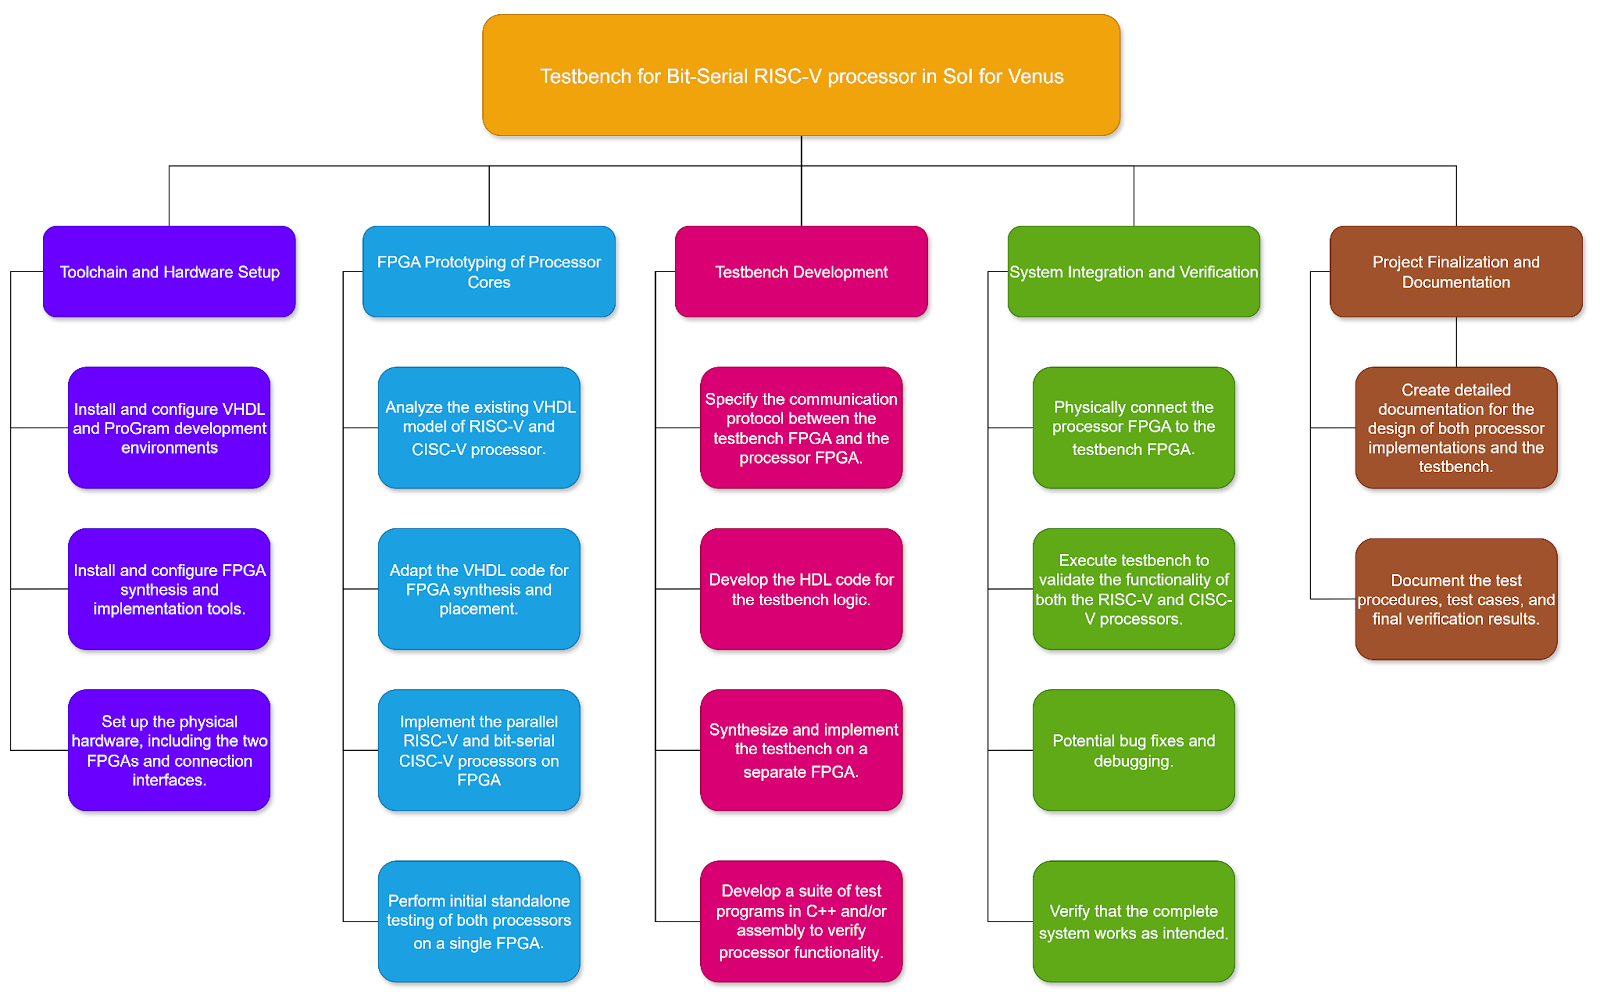
\includegraphics[width=\linewidth]{WBS.png}
\caption{Work Breakdown Structure (WBS)}
\label{fig:timeline}
\end{figure}

The main phases of the project are:
\begin{itemize}
  \item \textbf{Toolchain and Hardware Setup} : This initial phase involves preparing the necessary software environments and physical hardware for development and testing.
  \item \textbf{FPGA Prototyping of Processor Cores} : This phase focuses on adapting, implementing, and performing initial tests on the existing RISC-V and CISC-V processor models on an FPGA.
  \item \textbf{Testbench Development} : This involves designing and implementing the advanced testbench on a separate FPGA, which will be used to validate the processor cores.
  \item \textbf{System Integration and Verification} : This phase covers the physical connection of the two FPGAs and the execution of comprehensive tests to validate the complete system and debug any potential issues.
  \item \textbf{Project Finalization and Documentation} : The final phase includes creating detailed documentation for the designs and test procedures, and preparing the final project deliverables.
\end{itemize}
This structure provides a comprehensive overview of the project's scope and organizes all required work into logical, manageable packages.


\section{Global plan}

\begin{table}[h!]
\centering
\begin{tabular}{|l|l|l|}
\hline
\textbf{Week} & \textbf{Sprint Focus} & \textbf{Main Deliverable} \\ \hline
Week 41 (Oct 6–13) & Sprint 1 – Setup project environment, FPGA toolchain, GitHub structure & Project Plan \\ \hline
Week 42 (Oct 14–20) & Sprint 2 – Start testbench architecture & Early TB design \\ \hline
Week 43–44 & Sprint 3–4 – Integrate CISC-V with testbench, basic simulation & Status Report 1 \\ \hline
Week 45–46 & Sprint 5–6 – Implement and connect RISC-V, improve testbench & Status Report 2 \\ \hline
Week 47–50 & Sprint 7–9 – Hardware testing on FPGA, validation and debugging & TB verification results \\ \hline
Week 51–1 & Sprint 10–11 – Prepare documentation, lessons learned, final report & Final report \& presentation \\ \hline
\end{tabular}
\caption{Global sprint overview and deliverables for the project.}
\label{tab:sprint_overview}
\end{table}


\section{First sprint plan}

\end{document}
